\documentclass[a4paper,12pt]{article}
%\usepackage[latin1]{inputenc}
\usepackage[spanish]{babel}
\usepackage{bm}
\usepackage{graphicx}
\usepackage{amsmath}
\setlength{\textheight}{235mm}
\setlength{\textwidth}{168mm}
\setlength{\oddsidemargin}{0pt}
\pagestyle{empty}
\spanishdecimal{.}
\begin{document}
\mbox{}\vspace*{-45mm}

{\centering
{\small\sc Escuela Técnica Superior de Ingenieros de Caminos, Canales y
Puertos (Madrid)}\\*[4mm]
{\Large\bf Método de los Elementos Finitos (Curso 23-24)}\\*[4mm]
Práctica 2: Ecuación de difusión \\*[4mm]
}

\vspace{3mm}

%%%%%
\noindent
La figura muestra la sección transversal de un río canalizado, en una zona en la que se ha construido un túnel provisional de $5$ m de longitud y sección cuadrada de $1$ m de lado. El extremo derecho del túnel está a la presión atmosférica. El terreno tiene un coeficiente de permeabilidad $k=2\cdot10^{-3}$ m/s y está confinado por pantallas impermeables y terreno igualmente impermeable.

Para analizar las filtraciones que se producen se realizará un modelo plano de elementos finitos que represente dicha sección transversal. La discretización a efectuar corresponde a elementos cuadrados de cuatro
nodos de lado $0.25$ m.

Analizar la distribución de presiones (altura piezométrica) y la distribución de velocidades horizontales y verticales.

\begin{center}
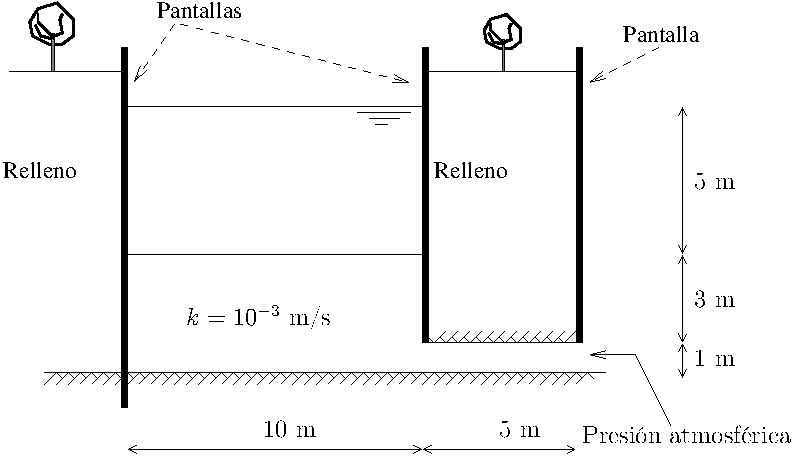
\includegraphics[width=0.75\textwidth]{practi2}
\end{center}

\end{document}
